\chapter{Probability and Statistics DV}

\textbf{Resorcess}
\begin{itemize}
    \item \url{https://www.falstad.com/circuit/circuitjs.html}
    \item \url{http://www.32x8.com/var4kmapx.html}
    \item \url{https://www.tinkercad.com/dashboard?type=circuits&collection=designs}
    \item \url{https://www.symbolab.com/solver/system-of-equations-calculator}
\end{itemize}

\newpage

\section{Circuit Theory}
\subsection{Basic electical quantities}
%https://www.khanacademy.org/science/electrical-engineering/introduction-to-ee
\subsubsection{Current}
$i (A)$: amps \newline

Positive repels Positiv. Negative repels Negative. Positive and Negative force of attraction.
Copper is commonly used in wires since there is only one electron in last orbital. This makes it easy
to move therefore it is higly conductive. \newline

$I = q^{-} / sec$ Current is charge per second. \newline

Current is writen from Positiv to Negative. Since back in history Ben Franklin who studied elektriesaty and
came up with theories. However the were unaware that electrons exsisted and there fore made the false
assumption that the current goese from positive to negative. With infact the electron is attracted to
the posiive end and therefore flows that way.
Ben Franklin $1747$.
JJ Thompson $1897$ $e^{-}$.
However positve chage dose exist like in your body then it would be true. \newline

Electron current is from negative to possitive. Conventional current (the current we know as) is from
positive to negative.

\subsubsection{Voltage}
$v (V)$: volt \newline
Voltage is simmular to gravity. It is the potential difference in the two pols, in otherwords
like potatial enegry like in the gravity analagy.

\begin{figure}[h]
    \vspace{10mm}
    \centering
    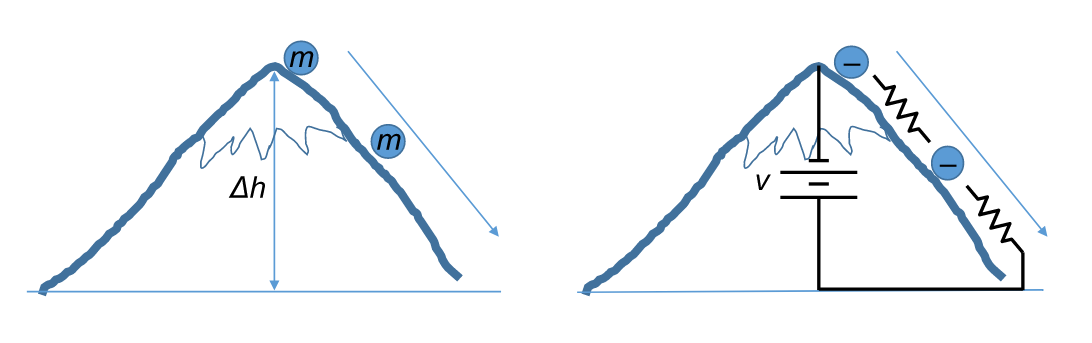
\includegraphics[width=15cm, height=6cm]{image/volt.png}
    \caption{volt}
\end{figure}

$V=\frac{\Delta{U}}{q}$ Where $\Delta{U}$ is the potational energy diffrent and $q$ is charge particle

\newpage
\subsubsection{Power}
Power is defined as the rate energy ($U$) is transformed or transferred over time. We measure power in units of joules/second, also known as watts.
$1$ watt = $1$ joules / second) \newline

An electric circuit is capable of transferring power. Current is the rate of flow of charge, and voltage measures the energy transferred per unit of charge. We can insert these definitions into the equation for power:
$p = \frac{dU}{dt} = \frac{dU}{dq} * \frac{dq}{dt}$. ($dU=\Delta{U}$)

\begin{equation} p = v*i \end{equation}

\subsection{Prefixes}
\begin{center}
\begin{tabular}{ c c c c }
 Number    & Prefix & Symbol & Note \\
 $10^{+10}$ & tera-  & $T$    &   \\
 $10^{+9}$  & giga-  & $G$    &   \\
 $10^{+6}$  & mega-  & $M$    &   \\
 $10^{+3}$  & kilo-  & $k$    & the only $> 1$ prefix in lower case \\
 $10^{0}$   &        &        &   \\
 $10^{-3}$  & milli- & $m$    &   \\
 $10^{-6}$  & micro- & $\mu$  &  be careful $\mu$ \(mu\) doesn't turn into "m" \\
 $10^{-9}$  & nano-  & $n$    &   \\
 $10^{-12}$ & pico-  & $p$    &   \\
\end{tabular}
\end{center}

\subsection{Unit grammar}
\begin{center}
\begin{tabular}{ c c c c c }
 Symbol name & example names & Symbol & example symbols & Named after \\
 second & 1 millisecond & $s$      & $2 ns$       &    \\
 meter  & 300 kilometer & $m$      & $35 nm35$    &    \\
 hertz  & 10 kilohertz  & $Hz$     & $100 MHz$    &  Hertz  \\
 ohm    & 2 megohm      & $\Omega$ & $47 k\Omega$ &  Ohm  \\
 farad  & 10 picofarad  & $F$      & $220 pF220$  &  Faraday  \\
 ampere & 35 microamp   & $A$      & $65 mA$      &  Ampère  \\
 volt   & 11 kilovolt   & $V$      & $5\mu{V}$    &  Volta  \\
\end{tabular}
\end{center}

%$e=-1.602176565*10^{-19}$ coulombe

\subsection{Ohm's law}
\begin{itemize}
  \item V (Voltage): V (volt)
  \item I (Current): A (amps)
  \item R (Resistance): $\Omega$ (omega)
\end{itemize}

\begin{equation} i = \frac{v}{r} \end{equation}


\subsection{Circuit elements}
%Elements are either sources or components.
\begin{figure}[h]
    \vspace{10mm}
    \centering
    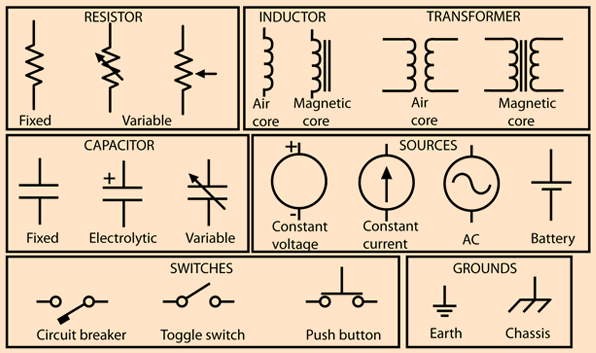
\includegraphics[width=10cm]{image/circuit-elements.png}
    \caption{\href{http://hyperphysics.phy-astr.gsu.edu/hbasees/Electronic/cktelcon.html}{Circuit elements}}
\end{figure}



%\subsubsection{Resistor}
%\begin{figure}[h]
%    \vspace{10mm}
%    \centering
%    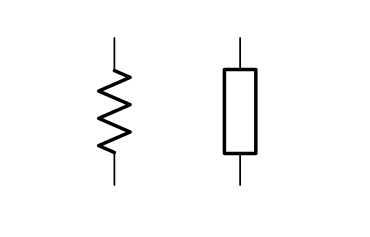
\includegraphics[width=5cm]{image/resistor.png}
%    \caption{resistor}
%\end{figure}
%
%\subsubsection{Capasitor}
%\begin{figure}[h]
%    \vspace{10mm}
%    \centering
%    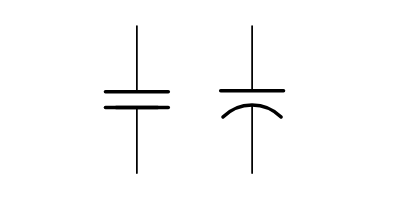
\includegraphics[width=5cm]{image/capacitor.png}
%    \caption{capacitor}
%\end{figure}
%
%\subsubsection{Inductor}
%\begin{figure}[h]
%    \vspace{10mm}
%    \centering
%    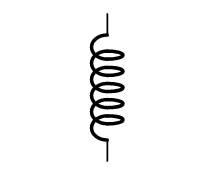
\includegraphics[width=5cm]{image/inductor.png}
%    \caption{inductor}
%\end{figure}
%
%\newpage
%\subsubsection{Ideal Soruce}
%Sources provide energy to a circuit. There are two basic types.\newline
%Voltage source
%\begin{figure}[h]
%    \vspace{10mm}
%    \centering
%    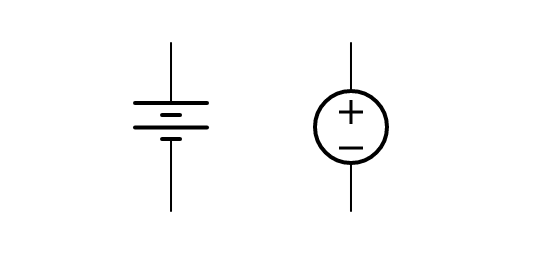
\includegraphics[width=5cm]{image/constant-voltage-source.png}
%    \caption{constant-voltage-source}
%\end{figure}
%
%Current source
%\begin{figure}[h]
%    \vspace{10mm}
%    \centering
%    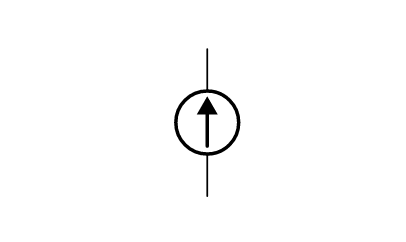
\includegraphics[width=6cm, height=3cm]{image/constant-current-source.png}
%    \caption{constant-current-source}
%\end{figure}


\newpage
\subsection{Circut termenology}
\begin{itemize}
    \item \textit{Closed circuit} – A circuit is closed if the circle is complete if all currents have a path back to where they came from.
    \item \textit{Open circuit} – A circuit is open if the circle is not complete if there is a gap or opening in the path.
    \item \textit{Short circuit} – A short happens when a path of low resistance is connected (usually by mistake) to a component. The resistor shown below is the intended path for current, and the curved wire going around it is the short. Current is diverted away from its intended path, sometimes with damaging results. The wire shorts out the resistor by providing a low-resistance path for current (probably not what the designer intended).
    \item \textit{Node} - Between elements
    \item \textit{Branch} - path between two noodes.
    \item \textit{Loop} - Close path in a circuit  (Branch - Nodes + 1)
\end{itemize}

\subsection{Series Resistor}
\begin{equation} R_{series} = R_1 + R_2 + \ldots + R_n \end{equation}

\begin{figure}[h]
    \vspace{10mm}
    \centering
    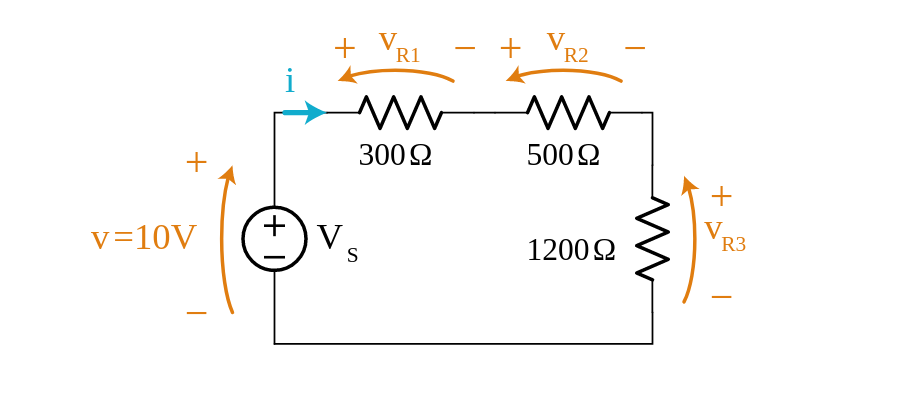
\includegraphics[width=7cm]{image/voltage-distributes-between-resistors-in-series.png}
    \caption{voltage distributes between resistors in series}
\end{figure}


\begin{align*}
  &\quad R_{series} = 300\Omega + 500\Omega + 1200\Omega = 2000\Omega \\
  &\quad i = \frac{v}{R_{series}} = \frac{10V}{2000\Omega} = 5mA \\
  &\quad \\
  &\quad v_{R1} = i\cdot R1 = 5mA\cdot 300\Omega = 1.5V \\
  &\quad v_{R2} = i\cdot R2 = 5mA\cdot 500\Omega = 2.5V \\
  &\quad v_{R3} = i\cdot R3 = 5mA\cdot 1200\Omega = 6.0V \\
  &\quad 10V -1.5V -2.5V -6.0V = 0V \text{ Therefore correct }\\
\end{align*}


\newpage
\subsection{Parralel resistor}
\begin{equation} \frac{1}{R_p} = \frac{1}{R_1} + \frac{1}{R_2} \end{equation}
\begin{equation} R_{parallel} = \frac{1}{\frac{1}{R_1} + \frac{1}{R_2}} \end{equation}

\begin{figure}[h]
    \vspace{10mm}
    \centering
    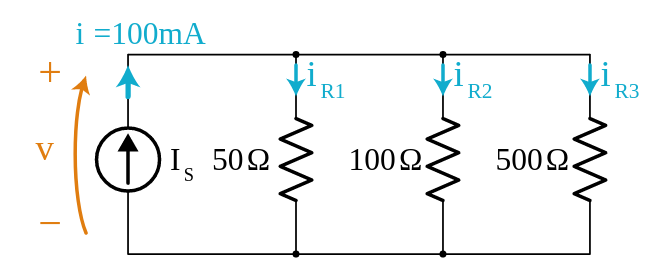
\includegraphics[width=6cm]{image/current-distributes-between-resistors-in-parallel.png}
    \caption{current distributes between resistors in parallel}
\end{figure}

\begin{align*}
  &\quad R_{parallel} = \frac{1}{\frac{1}{R_1} + \frac{1}{R_2} + \frac{1}{R_3}} \\
  &\quad R_{parallel} = \frac{1}{\frac{1}{0.02} + \frac{1}{0.01} + \frac{1}{0.002}} =
  \frac{1}{0.032} = 31.25\Omega \\
  &\quad v=i\cdot{R_{parallel}} = 100mA\cdot{31.25\Omega} = 3.125V \\
  &\quad \\
  &\quad i_{R1} = \frac{v}{R1} = \frac{3.125V}{50\Omega} = 62.5mA \\
  &\quad i_{R2} = \frac{v}{R2} = \frac{3.125V}{100\Omega} = 31.25mA \\
  &\quad i_{R3} = \frac{v}{R3} = \frac{3.125V}{500\Omega} = 6.25mA \\
  &\quad 100mA -62.5mA -31.25mA -6.25mA = 0mA \text{ Therefore correct }\\
\end{align*}


\subsection{Simplify resistor network}
\underline{Start} from the \underline{furthest point}. Make parallel and serial resistors become one.

\newpage
\subsection{Voltage divider}
\begin{figure}[h]
    \vspace{10mm}
    \centering
    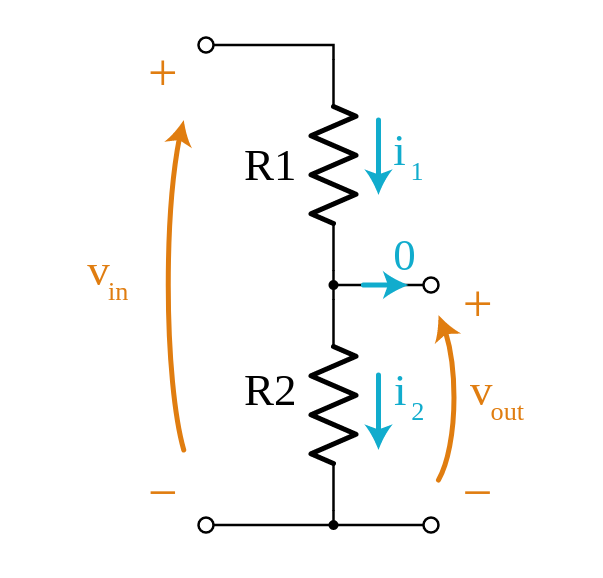
\includegraphics[width=8cm, height=6cm]{image/voltage-divider.png}
    \caption{voltage-divider}
\end{figure}

\begin{align*}
  v_{in} &= i(R_1+R_2) \Rightarrow I = \frac{1}{R_1+R_2}v_{in} \\
  v_{out} &= iR_2 \Rightarrow v_{out} = \frac{R_2}{R_1+R_2}v_{in} \\
  &= \frac{1}{\frac{R_1}{R_2}+1}v_{in}
\end{align*}

\subsection{Kirchhoff's laws}
\subsubsection{Kirchhoff's current law}
KCL
\begin{equation} \sum i_{in} = \sum i_{out} \end{equation}

\subsubsection{Kirchhoff's voltage law}
KVL
\begin{equation} \sum_n V_{n} = 0 \end{equation}
\begin{equation} \sum V_{rise} = V_{drop} \end{equation}


\newpage
\subsection{Node voltage method}
%https://www.khanacademy.org/science/electrical-engineering/ee-circuit-analysis-topic/ee-dc-circuit-analysis/a/ee-node-voltage-method
\begin{figure}[h]
    \vspace{10mm}
    \centering
    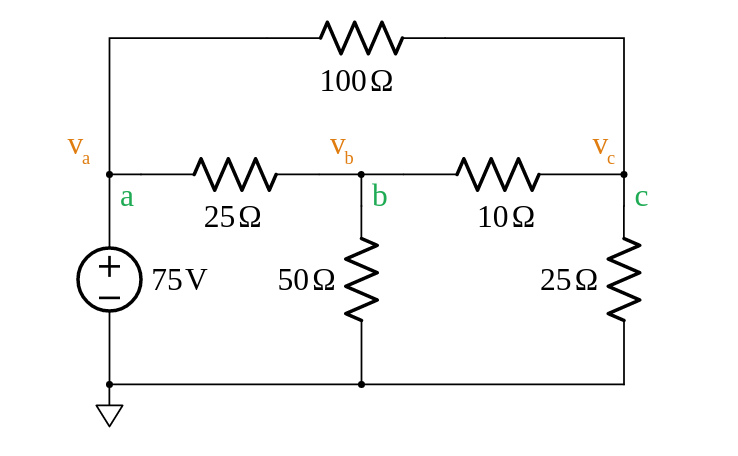
\includegraphics[width=10cm, height=6cm]{image/node-voltage-method.png}
    \caption{Example node voltage method}
\end{figure}


\begin{align*}
  &\quad 1. \textbf{ Assign a reference node (ground).} \\
  &\quad \text{Assign it under Voltage sorce} \\
  &\quad \\
  &\quad 2. \textbf{ Assign node voltage names to the remaining nodes.} \\
  &\quad \text{See imgage for } v_a, \; v_B, \; v_c, \; a, \; b, \; c  \\
  &\quad \\
  &\quad 3. \textbf{ Solve the easy nodes first, the ones with a voltage source connected to the reference node.} \\
  &\quad V_a \text{ is the easyest since it is the same as the input } v_a=75V \\
  &\quad \\
  &\quad 4. \textbf{Write Kirchhoff's Current Law for each node. Do Ohm's Law in your head.} \\
  &\quad \text{Node $b$: } +\frac{v_a-v_b}{25} -\frac{v_b}{50} +\frac{v_c-v_b}{10} = 0 \\
  &\quad \text{Node $c$: } +\frac{v_a-v_c}{100} -\frac{v_b-v_c}{10} +\frac{v_c}{25} = 0 \\
  &\quad \\
  &\quad 5. \textbf{Solve the resulting system of equations for all node voltages.} \\
  &\quad \text{Node $b$: } -\frac{v_b}{25} -\frac{v_b}{50} -\frac{v_b}{10} +\frac{v_c}{10} = -\frac{v_a}{25} \\
  &\quad \Rightarrow -\frac{8}{50}v_b +\frac{1}{10}v_c = -\frac{75}{25} = -3 \\
  &\quad \text{Node $c$: } +\frac{v_b}{10} -\frac{v_c}{100} -\frac{v_c}{10} +\frac{v_c}{25} = -\frac{v_a}{100} \\
  &\quad \Rightarrow +\frac{1}{10}v_b -\frac{15}{100}v_c = -\frac{75}{100} = -\frac{3}{4} \\
  &\quad \\
  &\quad \textbf{Solve by gauseelimination and then get } v_b=+37.5V, \: v_c=+30V \\
  &\quad \\
  &\quad 6. \textbf{Solve for any currents you want to know using Ohm's Law.} \\
  &\quad i_{ab25\Omega} = \frac{75-37.5}{25} = 1.5A  \text{ arrow pointing right} \\
  &\quad i_{bg50\Omega} = \frac{37.5}{50} = 0.75A    \text{ arrow pointing down} \\
  &\quad i_{bc10\Omega} = \frac{37.5-30}{10} = 0.75A \text{ arrow pointing right} \\
  &\quad i_{ac100\Omega} = \frac{75-30}{100} = 0.45A \text{ arrow pointing right} \\
  &\quad i_{cg25\Omega} = \frac{30}{25} = 1.2A       \text{ arrow pointing down} \\
  &\quad \\
\end{align*}

\newpage
\subsection{Mesh current method}
%https://www.khanacademy.org/science/electrical-engineering/ee-circuit-analysis-topic/ee-dc-circuit-analysis/a/ee-mesh-current-method
%https://www.khanacademy.org/science/electrical-engineering/ee-circuit-analysis-topic/ee-dc-circuit-analysis/a/ee-loop-current-method

\begin{figure}[h]
    \vspace{10mm}
    \centering
    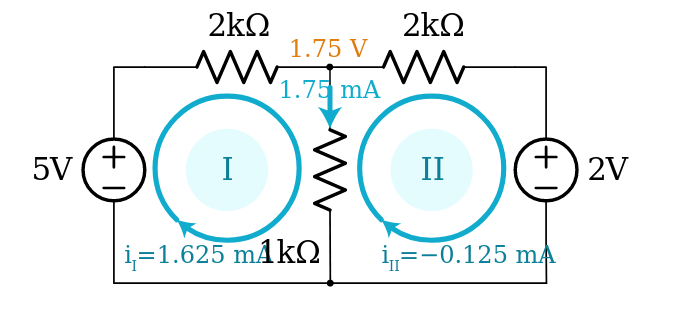
\includegraphics[width=12cm, height=6cm]{image/mesh_current_method.png}
    \caption{Mesh current method}
\end{figure}

\begin{align*}
  &\quad  \text{Mesh I: } \\
  &\quad  +\text{The voltage sorce} -\text{voltage drop over first resistor} 
  -\text{voltage over second resitor} = 0 \;\;\; \text{ (KVL)} \\
  &\quad  +5V -2000i_I -1000(i_I-i_{II}) = 0 \\
  &\quad  \\
  &\quad  \text{Mesh II: } \\
  &\quad  +\text{Voltage over first resistor} -\text{Voltage over second resistor} 
  -\text{Voltage sorce} \\
  &\quad  +1000(i_I-i_{II}) -2000i_{II} -2V = 0 \\
  &\quad  \\
  &\quad  \text{Gauseelimination gives us } i_{II} = -0.125mA, \; i_I = +1.625mA \\
\end{align*}


\subsection{\href{https://www.khanacademy.org/science/electrical-engineering/ee-circuit-analysis-topic/ee-natural-and-forced-response/a/ee-capacitor-equation-in-action}{Capacitor i-v equation}}
%https://www.khanacademy.org/science/electrical-engineering/ee-circuit-analysis-topic/ee-natural-and-forced-response/a/ee-capacitor-equation-in-action
\begin{equation}
  i=C\frac{dv}{dt}, \; v=\frac{1}{C}\int^T_0 idt + v_0 
\end{equation}
\begin{itemize}
    \item C is the capacitance, a physical property of the capacitor (ex: $10\mu F$)
    \item $\frac{dv}{dt}$ reate of change for volt over time (ex: $100 volts/second$)
\end{itemize}

\subsection{\href{https://www.khanacademy.org/science/electrical-engineering/ee-circuit-analysis-topic/ee-natural-and-forced-response/a/wmc-inductor-in-action}{inductor i-v equation}}
%https://www.khanacademy.org/science/electrical-engineering/ee-circuit-analysis-topic/ee-natural-and-forced-response/a/wmc-inductor-in-action
\begin{equation}
  v=L\frac{di}{dt}, \; \frac{1}{L}\int^T_0 vdt + i_0
\end{equation}
\begin{itemize}
    \item L is the inductance, a physical property of the inductor (ex: $1mH$)
    \item $\frac{di}{dt}$ is the reate of change for the current over time (ex: $300 ampere/second$)
\end{itemize}

\newpage
\subsection{RC circuit}
\subsubsection{\href{https://www.khanacademy.org/science/electrical-engineering/ee-circuit-analysis-topic/ee-natural-and-forced-response/a/ee-rc-natural-response}{RC natural response}}
%https://www.khanacademy.org/science/electrical-engineering/ee-circuit-analysis-topic/ee-natural-and-forced-response/a/ee-rc-natural-response
When initializes the circuit with a voltage and the capacitor will then be charged. Then we disconnect
the voltage source, the capasitor will act as a battary and edvenshula discharge. 
\begin{equation}
  v(t)=v_0e^{-t/RC}
\end{equation}
\begin{itemize}
    \item Time constant: $\tau=RC$. It is the time it takes to charge the capacitor, through the resistor.
    \item $v_0$ is the voltage at $t=0$
\end{itemize}

\textbf{Example:}
\begin{figure}[h]
    \centering
    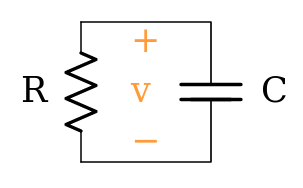
\includegraphics[width=5cm]{image/ex_RC_natural_response.png}
    \caption{EX RC natural response}
\end{figure}

\begin{align*}
  &\quad  \textbf{a. Write the expression for } v(t) \\
  &\quad  v(t) = V_0e^{-t/RC} = 1.4e^{-t/(3k\Omega\cdot{1\mu{F}}} 1.4e^{-t/3ms} \\
  &\quad  \textbf{b. What is $v(t)$ when $t=RC$?} \\
  &\quad  \tau=RC=3\times10^3\cdot{1\times10^{-6}} = 3ms \\
  &\quad  v(3ms) = 1.4e^{-3ms/3ms} = 1.4\cdot{1.4\cdot{0.3679}} = 0.515V \\
  &\quad  \textbf{c. Plot } v(t) \\
\end{align*}

\begin{figure}[h]
    \centering
    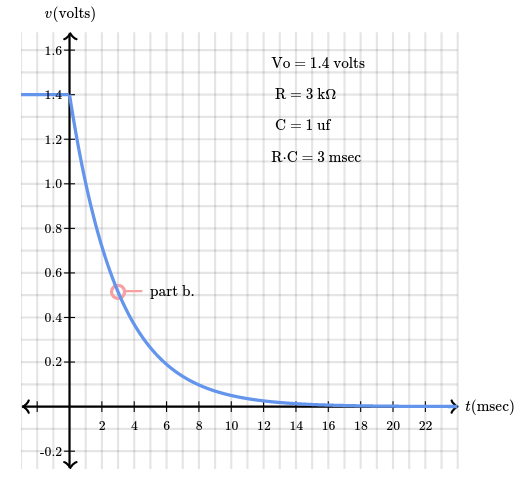
\includegraphics[width=7cm]{image/plot_RC_natural_response.png}
    \caption{Plot RC natural response}
\end{figure}

\newpage
\subsubsection{RC step response}
%https://www.khanacademy.org/science/electrical-engineering/ee-circuit-analysis-topic/ee-natural-and-forced-response/a/ee-rc-step-response
\begin{equation}
    \text{Total} = \text{Forced response} + \text{Natural response} 
\end{equation}
\begin{itemize}
    \item Foreced response: No start charge on capasitor and connected voltage supply
    \item Total responsee: what the circuit actoaly response.
\end{itemize}

\begin{equation}
  v(t) = V_s + (V_0-V_S)e^{-t/RC}
\end{equation}
\begin{itemize}
    \item $V_S$ is the height of the voltage step
    \item $V_0$ is the inital voltage on the capacitor
\end{itemize}

\subsubsection{LC natural response}
%https://www.khanacademy.org/science/electrical-engineering/ee-circuit-analysis-topic/ee-natural-and-forced-response/a/ee-lc-natural-response-derivation
\begin{equation}
  s^2 + 1/LC = 0
\end{equation}

\noindent\textbf{Euler's identities}
\begin{align*}
  e^{+jx} = \cos{x} + j\sin{x} \\
  e^{-jx} = \cos{x} - j\sin{x}
\end{align*}
where $j$ is the name for $\sqrt{-1}$

\noindent\textbf{Current function of time}
\begin{equation}
  i(t)=\sqrt{\frac{C}{L}}V_0\sin \omega_o t
\end{equation}

\noindent\textbf{Natural frequency of LC circuit}
\begin{equation}
  \omega_0 \equiv  \sqrt{\frac{1}{LC}}
\end{equation}

%https://www.khanacademy.org/science/electrical-engineering/ee-circuit-analysis-topic/ee-natural-and-forced-response/a/ee-lc-natural-response-derivation

\subsubsection{RLC}
The RLC end text circuit is the electronic equivalent of a swinging pendulum with friction.
\begin{equation}
  s = \frac{-R\pm\sqrt{R^2-4L/C}}{2L}
\end{equation}

\begin{equation}
  s = -\alpha  \pm \sqrt{\alpha^2 - \omega^2_o}
\end{equation}
where $\alpha=\frac{R}{2L}$ and $\omega_o=\frac{1}{\sqrt{LC}}$

\newpage
\section{Aplifier}
Saturates mean that it will become a state line since it can not become more than the input nor can it be less than what is going in the opposite direction.
$v_0=A(v^+-v^-)$ \newline

The current to $v^-$ and $v^+$ will be close to zero and in an ideal circuit will
be zero. \newline
%We can set $v_-=v_+=0$ when we know that the input is, ex $v_{in}$ is the input with is directly dependent on $v_{out}$ like in a feedback loop.
We can say $v^- = v^+$ when there is a feedback loop (negative terminal and noninverting amp). 

\subsection{Inside Op-Amp}
\begin{figure}[h]
    \vspace{10mm}
    \centering
    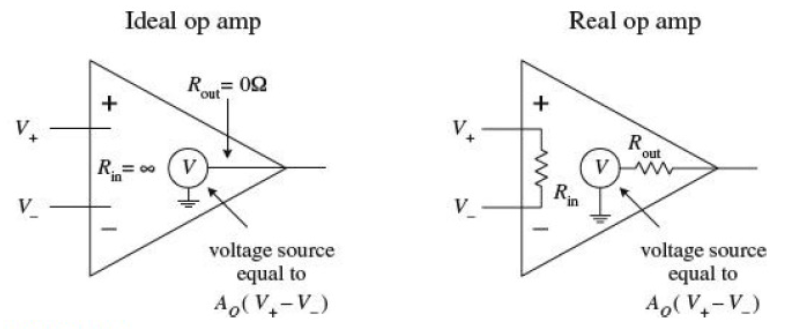
\includegraphics[width=12cm, height=6cm]{image/inside-opamp.png}
    \caption{Inside opAmp}
\end{figure}
In ideal op amp the resistancce will be infinity. However the in realaty
there is not infinit resistance therfore if one would have a voltage devider
with larger resistanse then the internal resistanse the current will 
go threw $V_+$ and $V_-$. The output in $0\Omega$ so we will not have any
voltage drop, not in reality however.

\newpage
\subsection{Implementation of Op-Amp}
\subsubsection{Comparator}
An op amp without negative feedback (a comparator)
\begin{figure}[h]
    \vspace{10mm}
    \centering
    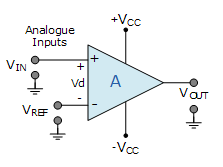
\includegraphics[width=8cm, height=6cm]{image/op-amp-comparator.png}
    \caption{Op-Amp comparator}
\end{figure}

When $V_+>V_-$ then $V_o=+V_{cc}$. When $V_+<V_-$ then $V_o=-V_{cc}$

\subsubsection{Non inverting (with feedback loop)}
Amplefies the input but dose not change it sign (non inverting).
An op amp with negative feedback (a non-inverting amplifier)

\begin{figure}[h]
    \vspace{10mm}
    \centering
    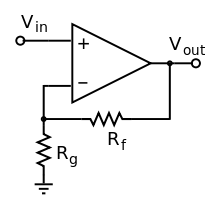
\includegraphics[width=6cm, height=6cm]{image/Operational_amplifier_noninverting.png}
    \caption{Op-Amp Feedback (Non inverting)}
\end{figure}

\newpage
\subsubsection{Voltage follower}
\begin{figure}[h]
    \vspace{10mm}
    \centering
    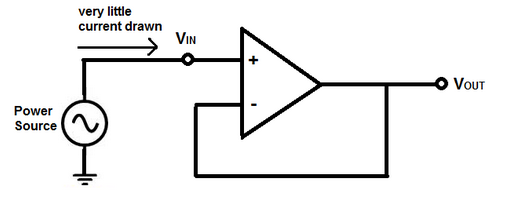
\includegraphics[width=12cm, height=6cm]{image/op-amp-voltage-follower.png}
    \caption{Op-Amp voltage follower}
\end{figure}
$v_+=v_-=v_{in}=v_{out}$

\newpage
\subsubsection{Inverting}
\begin{figure}[h]
    \vspace{10mm}
    \centering
    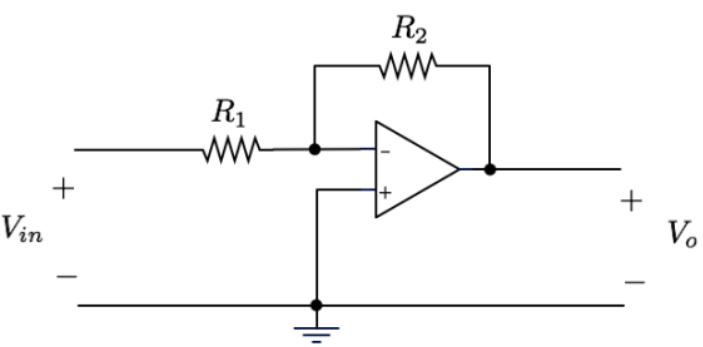
\includegraphics[width=8cm, height=6cm]{image/op-amp-inverting.png}
    \caption{Op-Amp voltage follower}
\end{figure}

\begin{figure}[h]
    \vspace{10mm}
    \centering
    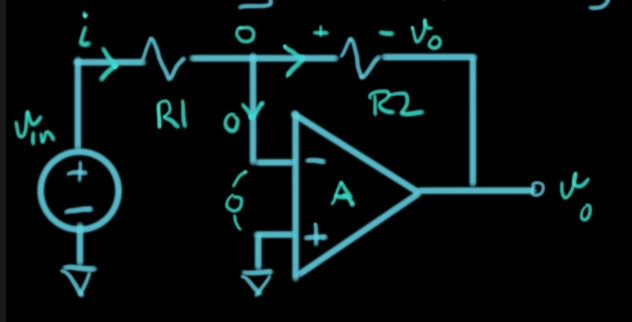
\includegraphics[width=10cm, height=6cm]{image/op-amp-calc-inverting.png}
    \caption{Op-Amp calculations for inverting}
\end{figure}
As seen from the image the current will be $i=v_{in}/R_1$ and $i=-v_0/R_2$. We combined them and get:
$V_0=\frac{-R_2}{R_1}V_{in}$

\newpage
\subsubsection{Summing}
\begin{figure}[h]
    \vspace{10mm}
    \centering
    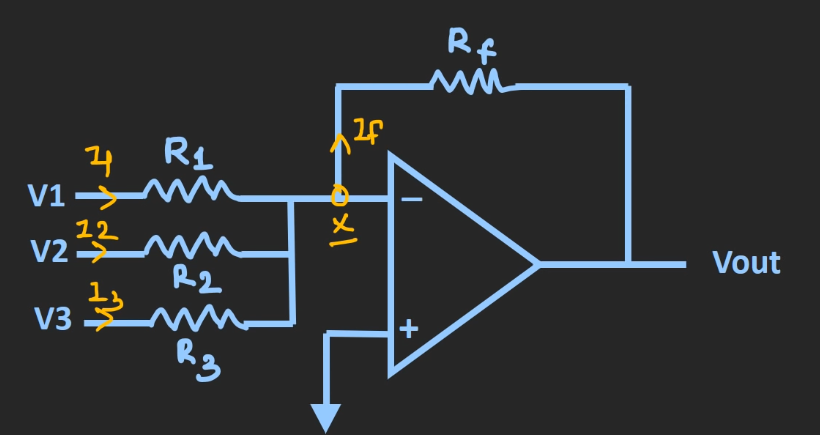
\includegraphics[width=8cm, height=6cm]{image/op-amp-summing.png}
    \caption{Op-Amp summing}
\end{figure}

Appling KCL we get: $I_f=I_1+I_2+I_3$ 
$\frac{v_1-0}{R_1} + \frac{v_2}{R_2} + \frac{V_3}{R_3} = \frac{0-v_{out}}{R_f}$
$\Rightarrow v_{out}=-(\frac{R_f}{R_1}V_1 + \frac{R_f}{R_2}V_2 + \frac{R_f}{R_3}V_3)$

\newpage
\subsection{Gerneral example}
\begin{figure}[h]
    \vspace{10mm}
    \centering
    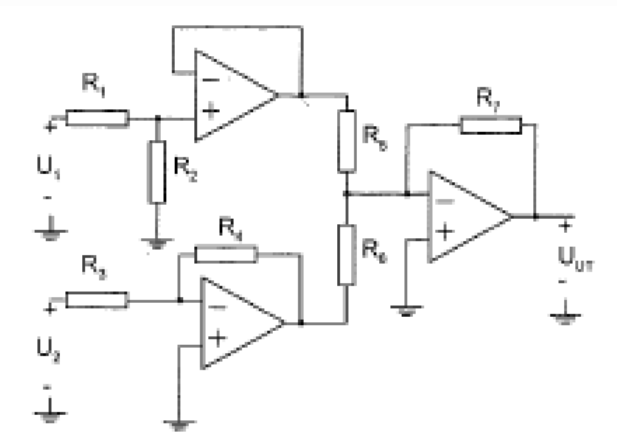
\includegraphics[width=8cm, height=6cm]{image/op-amp-example.png}
    \caption{Op-Amp example}
\end{figure}
\textbf{General opservations:} 
We can divide the circuit into three pieces. The one on the top is a   
\textit{Voltage follower}, we can call it circuit 1. The one on the bottom
is a \textit{Inverting op-amp} as is the middle one. We can name the bottom
one circuit 2 and the middle one is circuit 3.
\vspace{3mm}

\textbf{We start with circuit 3:} \newline
We name node \textbf{A} between $R_5$ and $R_6$. KCL: $I=I_5+I_6$ and $I=I_7$ since \newline
there is no current in $-$ terminal. \newline
$I=\frac{-U_{ut}}{R_7}=I_5+I_6=\frac{v_{O1}}{R_5}+\frac{v_{O2}}{R_6}$ \newline
Because of Ohm's law and $v_{over resistor}=v_{head}-v_{tail}$. \newline
\vspace{3mm}

\textbf{To solve $v_{O1}$ we need to solve circuit 1:} \newline
Applying KCL between $R_1$ and $R_2$ we get $I_1=I_2+I_3$ were $I_3=0$ since \newline
there is no current going in the $+$ terminal. $I_1=I_2$ Ohm's law result in \newline
$\frac{U_1-v_{O1}}{R_1}=\frac{V_{O1}-0}{R_2}$ since in a voltage follow circuit \newline
$v^-=v^+=v_{out}$. We then get $v_{out}=\frac{R_2}{R_1+R_2}U_1$ \newline
then $I_5=\frac{R_2}{(R_1+R_2)R_5}U_1$. \newline
\vspace{3mm}

\textbf{To solve $v_{O2}$ we need to solve circuit 2:} \newline
KCL gives $I_3=I_4$ since there is no current in $-$ terminal. \newline
Ohm's law $\frac{U_2-v^-}{R_3}=\frac{v^--v_{O2}}{R_4}$. \newline
$v^-=v^+=0$ with result in $\frac{U_2}{R_3}=\frac{-v_{O2}}{R_4}$. \newline
$v_{O2}=\frac{-R_4}{R_3}U_2$ \newline
The current $I_6=\frac{-R_4}{R_3R_6}U_2$ \newline
\vspace{3mm}

\textbf{Going back to circuit 3:} \newline
$I=I_5+I_6=\frac{R_2}{(R_1+R_2)R_5}U_1+\frac{-R_4}{R_3R_6}U_2$ \newline
results in $\frac{-U_{ut}}{R_7}=\frac{R_2}{(R_1+R_2)R_5}U_1+\frac{-R_4}{R_3R_6}U_2$. \newline
Finnal result: $U_{out}=-R_7(\frac{R_2}{R_5(R_1+R_2)}U_1-\frac{R_4}{R_3R_5}U_2)$

\newpage
\section{Semiconductors}
\subsection{Diodes}
\subsubsection{Ideal diodes}
Cundoct electrisity only one way. Current flowes threow Anode (A) to Cathode (K).
\begin{figure}[h]
    \centering
    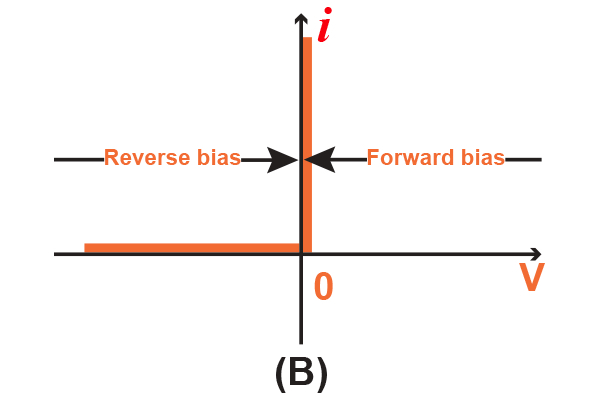
\includegraphics[width=8cm, height=6cm]{image/ideal-diode.jpg}
    \caption{ideal diode iv-curv}
\end{figure}

\subsubsection{Real diodes}
\textbf{reverse brakedown} is when the diode lets negative current. 
On normal diodes it will perminantly fail, probably melts.
\begin{equation}
  i=I_s(e^{qv_d/kT}-1)
\end{equation}
\begin{itemize}
  \item  $k$ is boltsmans constant ($1.38*10^{-23}J/K$ Jouls/Kelvin) $0K=-273^oC$
  \item  $T$ is tempreture of device (kelvin)
  \item  $I_s$ is structual current (silicon $10^{-12}A$), the small reverse current
  \item  $q$ is the charge of an electron ($1.1609*10^{-19}C$)
\end{itemize}

Difficult to use formula unless numerical analasys.

\begin{figure}[h]
    \centering
    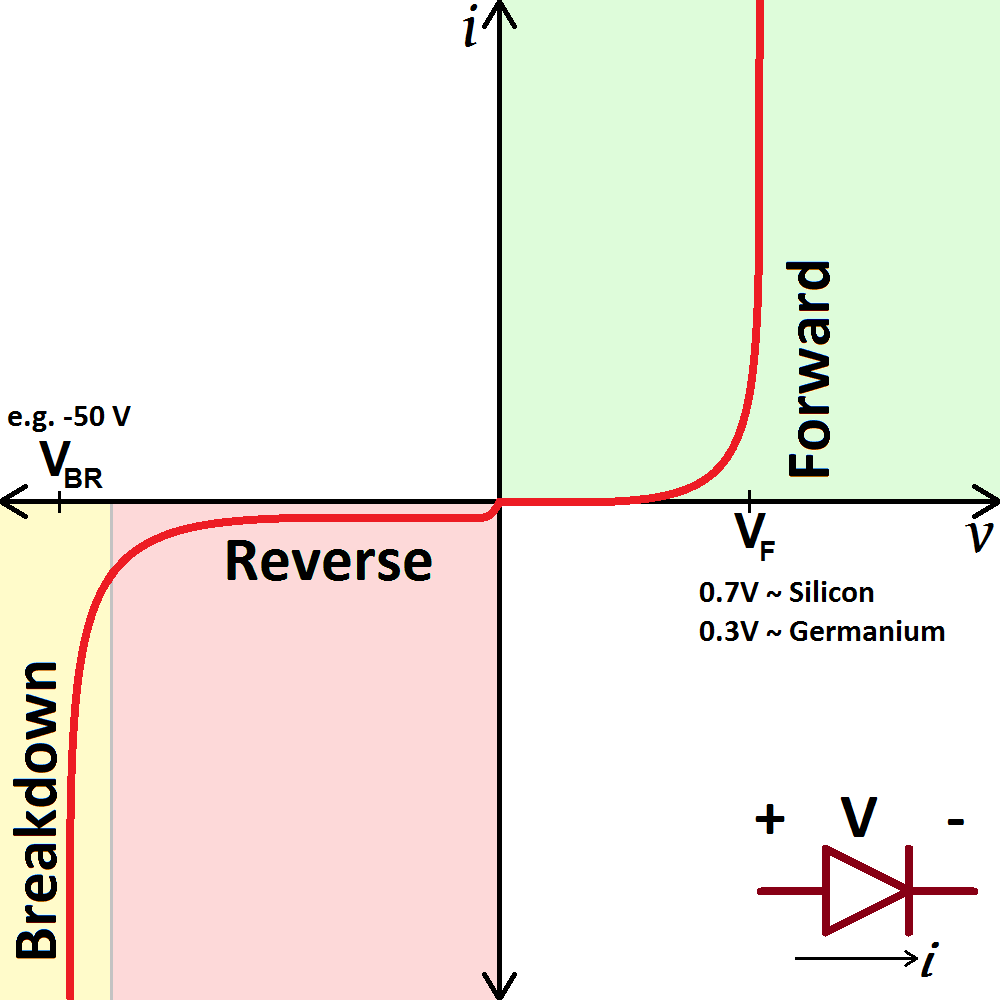
\includegraphics[width=8cm, height=6cm]{image/real-diode.png}
    \caption{real diode iv-curv}
\end{figure}

\newpage
\textbf{The DC model of a diode}
\begin{figure}[h]
    \centering
    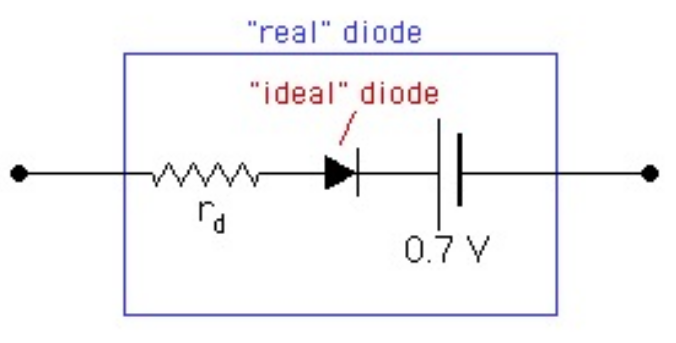
\includegraphics[width=8cm, height=6cm]{image/real_diode_dc.png}
    \caption{real diode dc model}
\end{figure}

\newpage
\textbf{Example: diode}
\begin{figure}[h]
    \centering
    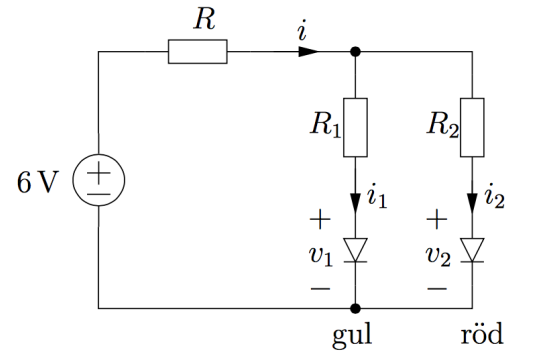
\includegraphics[width=8cm]{image/example-diode.png}
    \caption{diodes example}
\end{figure}

\begin{align*}
    &i_1 = 40mA, v_1 = 2v \\
    &i_2 = 50mA, v_2 = 1.6v \\
\end{align*}

\begin{align*}
    \text{Kirchhoffs strömlag: }& i=i_1+i_2=40mA+50mA=90mA=0.09A \\
    \text{Kirchhoffs spänningslag: }& \text{(Loop 1)} \\
    &+6-iR-R_1i_1-2=0 \\
    \text{Kirchhoffs spänningslag: }& \text{(Loop 2)} \\
    &+6-Ri-R_2i_2-1.6=0 \\
    \text{Vi har 3 okända och 2 eqvationer.}
    &\text{Närmed så kan vi sätta ett värde på R} \\
    \text{sådant att motstånden är} &\text{störe än noll} \\
    &R=20\Omega \Rightarrow R_1 = 55\Omega; R_2 = 52\Omega \\
\end{align*}



\newpage
\subsubsection{Zener Diodes}
Allows to enter and reenter the revese breakedown with out perminantly failing.
symbol. Jusaly lower voltage for revese breakdown
used for analog to digital conversion and vise versa and a voltage relulator.
%Un regulated voltage supply may be a dc voltage surce with varing output.
\begin{figure}[h]
    \centering
    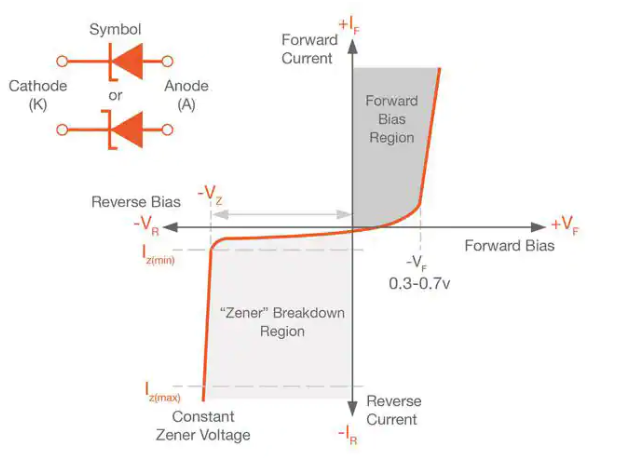
\includegraphics[width=8cm]{image/zener-diode.png}
    \caption{zener diode iv-curv}
\end{figure}

\begin{figure}[h]
    \centering
    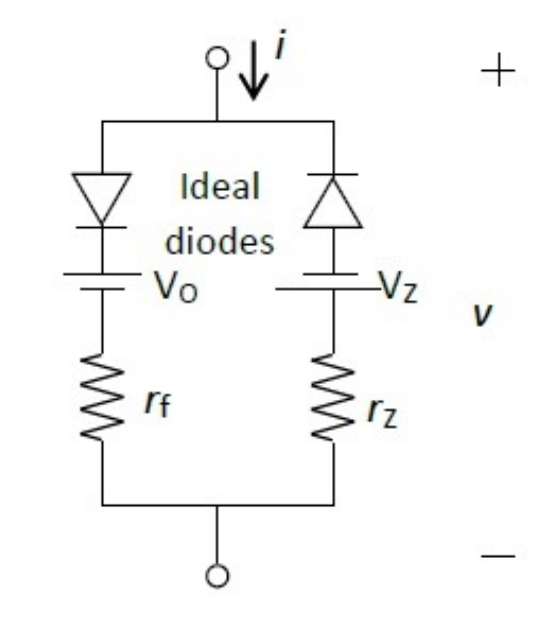
\includegraphics[width=7cm]{image/zener_diode_dc.png}
    \caption{zener diode dc model}
\end{figure}

\newpage
\textbf{Example}
Let $V_{in}=9V$ and $V_z=5V$. Determent the minimum value of $R$ if 
the maximum current is $20mA$ threw $R$, assume $R_L=\inf$. 
Then determan the minimum resistance for $R_L$
\begin{figure}[h]
    \vspace{10mm}
    \centering
    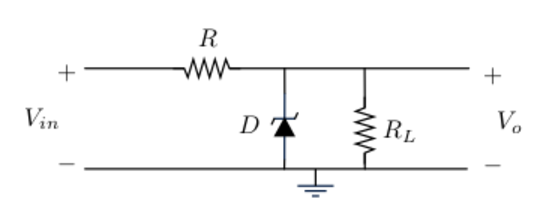
\includegraphics[width=8cm]{image/example_zener-diode.pdf}
    \caption{zener diode example}
\end{figure}

Let $I$ be the current over $R$, $I_1$ the current over the zener diode
and $I_2$ be the current over $R_L$.
\begin{align*}
    I &= \frac{V_{in}-V_o}{R} \\
    &\Rightarrow R > \frac{9-5}{20\cdot10^{-3}}\Omega = 200\Omega \\ 
    \\
    \text{KCL: }  I &= I_1 + I_2 \\
    I_1 &= 0 \; \text{ if $R_L$ is to low} \\
    I_2 &= \frac{V_0-0}{R_L} \\
    &\Rightarrow I = I_2 \Rightarrow 20mA = \frac{5v}{R_L} \\
    &\Rightarrow R_L > \frac{5}{20\cdot10^{-3}}\Omega = 250\Omega \\
\end{align*}


\newpage
\subsection{Transistors}
All Semiconductors are non linuer. But we can use transistors with linjer modules. \newline
NPN and PNP symbols. Base (B), Collector (C) and Emitter (E)
%how it behaves within a circuit
%Oporating point is the intersection of transistor curv and the line from kvl (in an aplifier ciruit)
% Liner model: (Cutoff (It is like an open circuit) V_{BE}<0.5V, i_B=0, i_C=0), (Saturation (we cant go any therder, top point curv), (Active (Horisontal line)))
% Amplifier is design to have the transistor in the acctive region. 
\begin{figure}[h]
    \vspace{10mm}
    \centering
    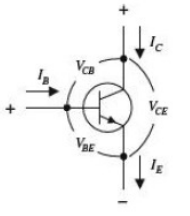
\includegraphics[width=6cm, height=6cm]{image/transistor-NPN.png}
    \caption{Transistor NPN}
\end{figure}

\begin{figure}[h]
    \vspace{10mm}
    \centering
    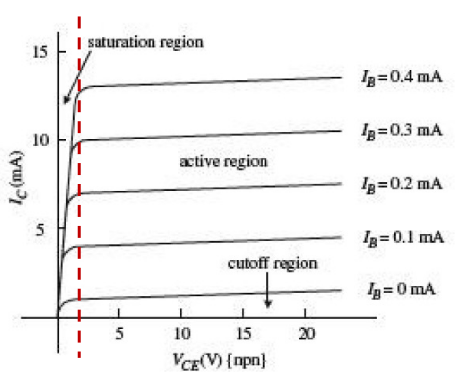
\includegraphics[width=7cm, height=6cm]{image/transistor_operation-mode.png}
    \caption{Transistor Operational mode}
\end{figure}


\newpage
\subsubsection{Transistor modes}
\noindent\textbf{Cutoff:}
Open switch
\begin{align*}
    &I_B = I_E = I_C = 0 \\
    &V_{BE}, \; V_{BC} < 0 \\
\end{align*}

\noindent\textbf{Saturation:}
Closed switch
\begin{align*}
    &V_{CE} <= V_{CEsat}, I_B>0 \\
\end{align*}

\noindent\textbf{Active:}
Dependent current source
\begin{align*}
    &I_E = I_B + I_C, \; I_C = h_{EF} I_B = \beta I_B \\
    &V_{CE} > V_{CEsat}, I_B>0, V_{BC} = V_B-V_C < 0 \\
\end{align*}


%\newpage
%\subsubsection{Field Effect Transistor (FET)}
%Manly two types Junktion Field Effect Transistor (JFET) and Metal Oxide Semiconductor Field Effect Transistor (MOSFET)
%The behaviur slightly diffrent from transisors.
%
%\textbf{JFET} has four pins \textit{Drain, Gate, Source} and \textit{Body}. 
%Body is allwase connected to source therefore symbol is still 3pin.
%There is intern two types off JFET N-chanel and P-channel.
%\textit{Pinch off} voltage is when There is no electrons flowing from source to drain.
%% are n/P-channel the oposit to echother VGS negative/positive
%N is in the middle for n-channel and P in a p-channel
%\begin{figure}[h]
%    \vspace{10mm}
%    \centering
%    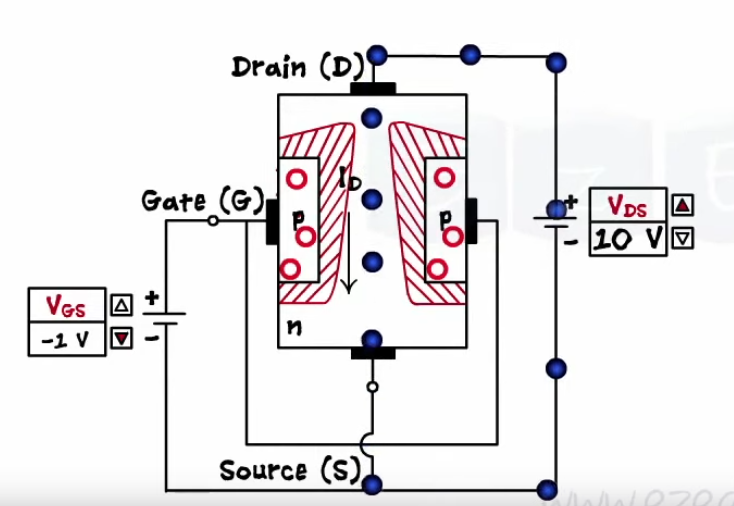
\includegraphics[width=8cm, height=6cm]{image/FET.png}
%    \caption{JFET}
%\end{figure}
%
%\textbf{MOSFET} has two types \textit{Enhancment (N-Channel)} and \textit{Depletion}. 
%It has the same pin careteristics as with JFET
%\begin{figure}[h]
%    \vspace{10mm}
%    \centering
%    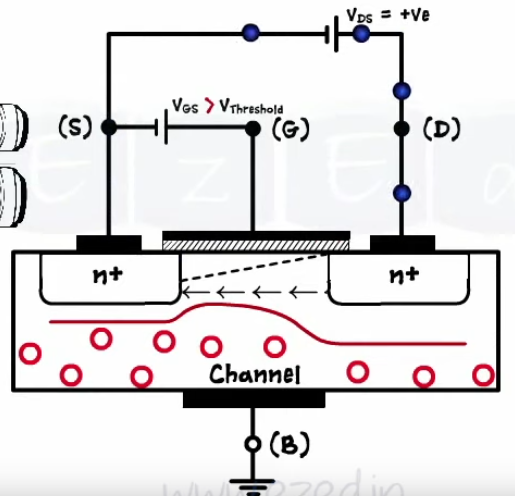
\includegraphics[width=7cm, height=6cm]{image/MOSFET.png}
%    \caption{MOSFET}
%\end{figure}
%
%\newpage
%The behaviur of a \textbf{FET} is:
%\begin{center}
%\begin{tabular}{ |c|c| } 
%  \hline
%  Cut off region & open switch \\
%  \hline
%  Active region & Amplifier \\
%  \hline
%  Saturation region & Closed switch \\
%  \hline
%\end{tabular}
%\end{center}

\textbf{Example: Transistor}
What is the larges value tjat $R_B$ can have so that the transistor 
behaves as a switch (saturation mode)? The transistor has a current gain
$h_{FE}$ between 100 and 300. Suppose that $V_{CE,sat}=0.2V$ and
$V_{BE,sat}=0.7$.
\begin{figure}[h]
    \centering
    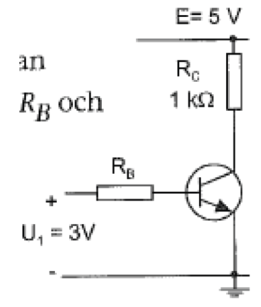
\includegraphics[width=4cm]{image/example-transistor.png}
    \caption{Transitor example}
\end{figure}

Om transistorn är bottnad (max current) gäller det att potatialen i C (mellan $R_C$
och transistorn)
\begin{align*}
    V_{CE} &= V_C - V_E = V_C - 0 = V_{CE,sat} \\
    V_C &= V_{CE,sat} = 0.2V
\end{align*}

$\Rightarrow$ Vi har då ett spänningsfall över $R_C$ på $5-0.2=4.8V$. \newline
\begin{align*}
    R_C\cdot I_C = 4.8V \;\; \text{ Ohm's law} \Rightarrow I_C = \frac{4.8}{10^3} = 4.8mA
\end{align*}

Vi vet att $I_C=\beta\cdot I_B$ men är ej säkra på $\beta$:s värde. Det kan vara så 
långt som 100. \newline

Vi kan behöva $I_B=\frac{I_C}{100}=48\mu A$ för att inte $I_C$ ska bli för liten.
Alltså: $I_B>48\mu A$ för att garantera bottnad transistor. \newline

Betrakta nu slingan där $I_B$ går. \newline
Potentialvandring: $U_1-R_BI_B-V_{BE,sat}= 0$, $3-R_BI_B-0.7=0$ \newline
eller $2.3=R_BI_B \Leftrightarrow I_B=\frac{2.3}{R_B}$ \newline

Använd olikhet $I_B>48\mu A \Rightarrow \frac{2.3}{R_B}>48\mu A$ $\Rightarrow \frac{2.3}{48\cdot10^{-6}}>R_B$ eller $R_B<47.9k\Omega$



\newpage
\section{Digital Circuits: Combinatorial and Sequential Networks}
\begin{figure}[h]
    \vspace{10mm}
    \centering
    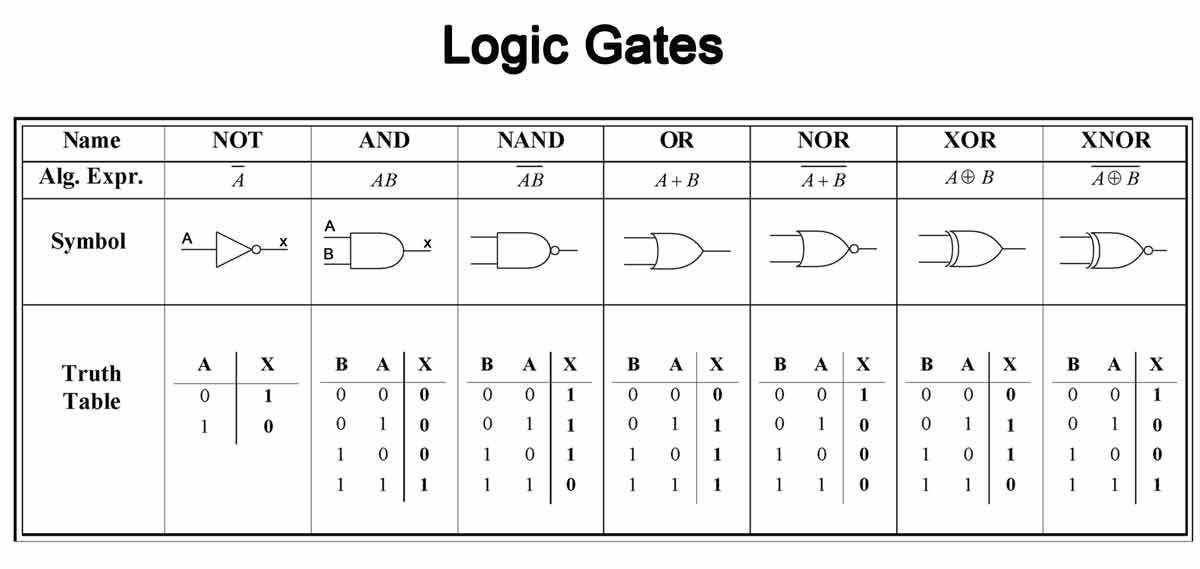
\includegraphics[width=10cm, height=6cm]{image/logic-gates.jpeg}
    \caption{Logic Gates}
\end{figure}

\textbf{Bolean algebra}
(or: $+$), (and: $\cdot$)
\[
\begin{aligned}
  x + x       &= x \\
  x \cdot x   &= x \\
  &\quad   \\
  x + x'      &= 1 \\
  x \cdot x'  &= 0 \\
  &\quad   \\
  x + 1       &= 1 \\
  x \cdot 0   &= 0 \\
  &\quad   \\
  x + 0       &= x \\
  x \cdot 1   &= x \\
\end{aligned} \qquad
\begin{aligned}
  (x')'       &= x \\
  &\quad   \\
  x + (y + x) &= (x +y) + z \\
  x(yz)       &= (xy)z \\
  &\quad   \\
  x(y+z)      &= xy+xz \\
  x + yz      &= (x+y)(x+z)   \\
  x + xy      &= x  \\
  &\quad   \\
  xy+\overline{x}z &= xy+\overline{x}z +yz  \\
  (x+y)(\overline{x}+z) &= (x+y)(\overline{x}+z)(y+z)   \\
  \overline{(x+y)} &= \overline{x}\overline{y}  \\
  \overline{(xy)} &= \overline{x}+\overline{y}  \\
\end{aligned}
\] 

\newpage
\subsection{Combinational}
$f(x_6,x_5,x_4,x_3,x_2,x_1,x_0) = x_6x_4(x_5+x_3+x_0) + x_2x_1$
\begin{figure}[h]
    \centering
    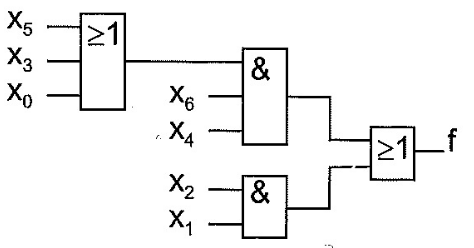
\includegraphics[width=6cm]{image/bolean-factorization.png}
    \caption{Bolean factorization}
\end{figure}

\begin{figure}[h]
    \centering
    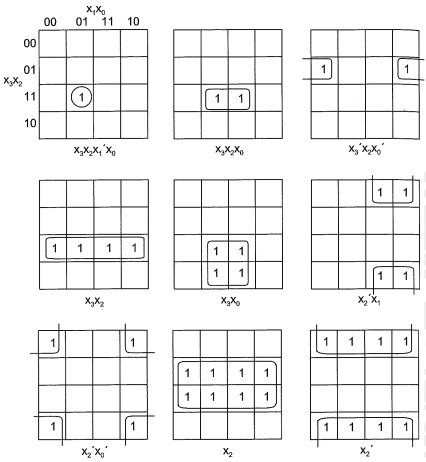
\includegraphics[width=5cm]{image/kmap-patterns.png}
    \caption{KMap patters}
\end{figure}
KMaps works from 4 variables.

\textit{Delays}, there is a small delay for each gate.

%implisent and explicet multiplicationo
%

\begin{figure}[h]
    \centering
    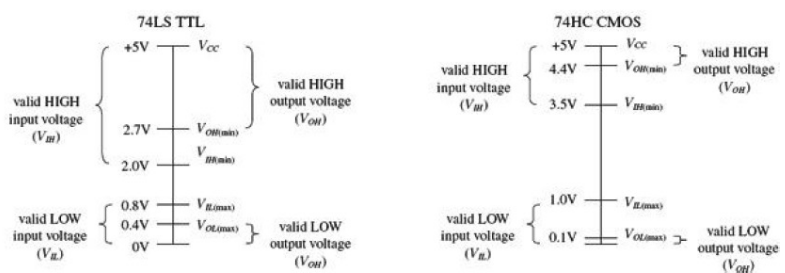
\includegraphics[width=12cm]{image/logic-families.png}
    \caption{Logic families}
\end{figure}

\newpage
\textbf{Example: desing circuit}
\begin{equation}
    f(x_3,x_2,x_1,x_0) = \sum(0,2,4,5,6,7) + d(8,10,12,14) \;\; \text{ - sum-of-products}
\end{equation}

\[
\begin{aligned}
     0 &= 0000 \\
     2 &= 0010 \\
     4 &= 0100 \\
     5 &= 0101 \\
     6 &= 0110 \\
     7 &= 0111 \\
     \\
     8 &= 1000 \\
    10 &= 1010 \\
    12 &= 1100 \\
    14 &= 1110 \\
\end{aligned} \qquad\qquad
\begin{aligned}
\begin{karnaugh-map}
   \manualterms{1,0,1,0,1,1,1,1,-,0,-,0,-,0,-,0}
   \implicant{4}{6}
   \implicantedge{0}{8}{2}{10}
\end{karnaugh-map}
\end{aligned}
\]

\begin{equation}
    f= \overline{x_0} + \overline{x_3}x_2    
\end{equation}

\begin{figure}[h]
    \centering
    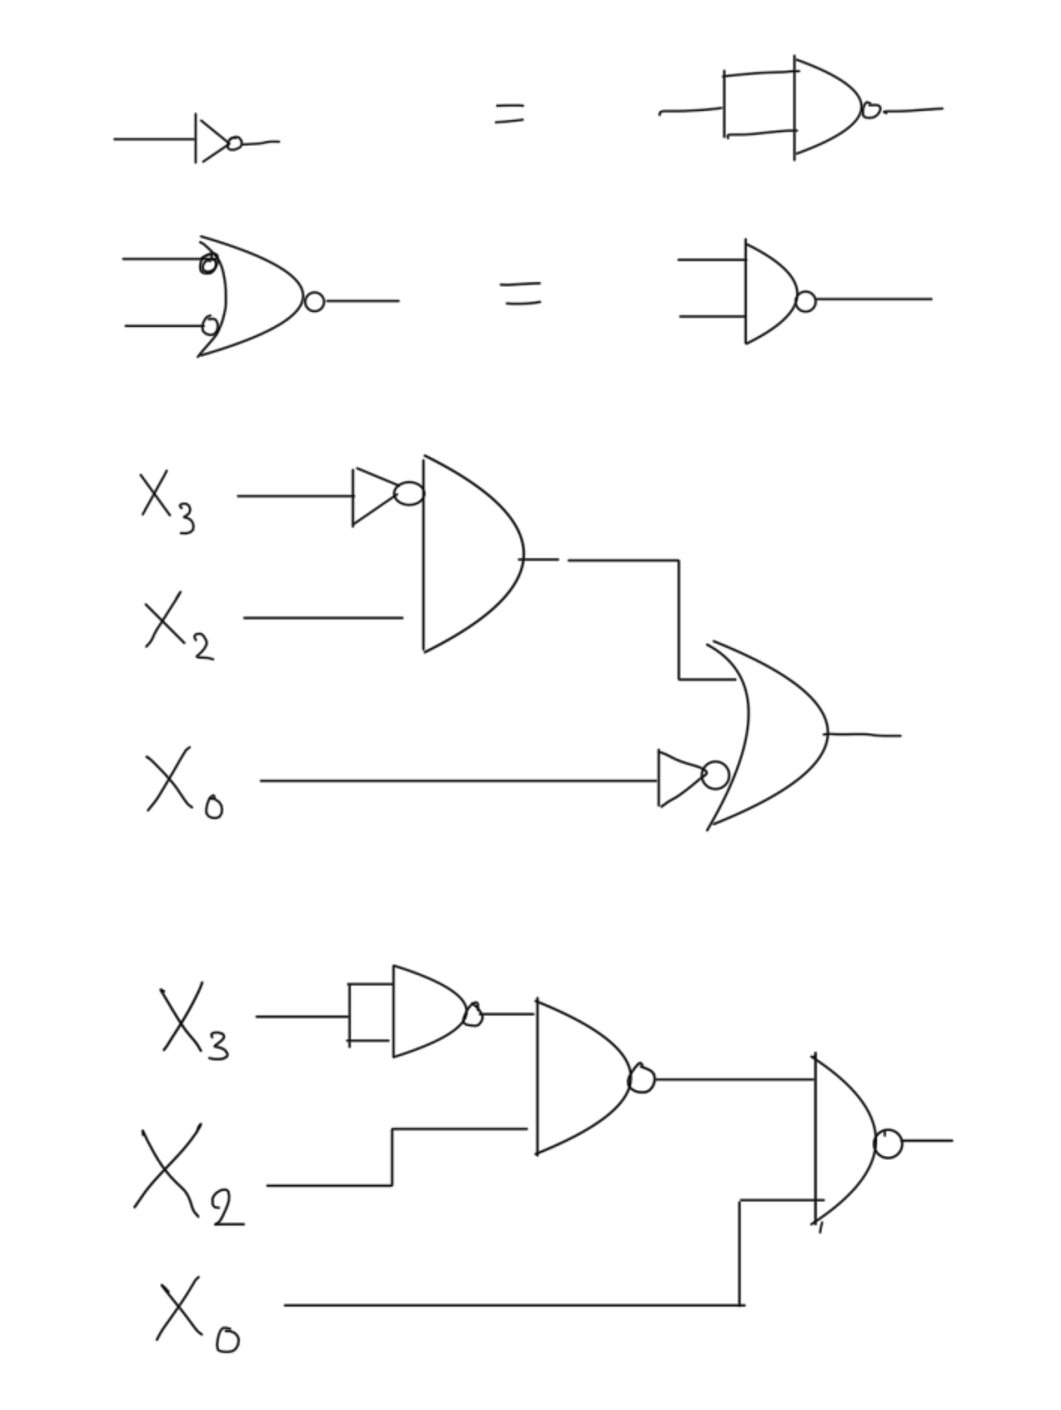
\includegraphics[width=8cm]{image/example-cobinational-lodgic.pdf}
    \caption{lodgic Combinational lodgic}
\end{figure}
 
%why is it slower to have a single gate with multiple input?

\newpage
\subsection{Sequential}
Remembers the state what happend before.

\begin{figure}[h]
    \centering
    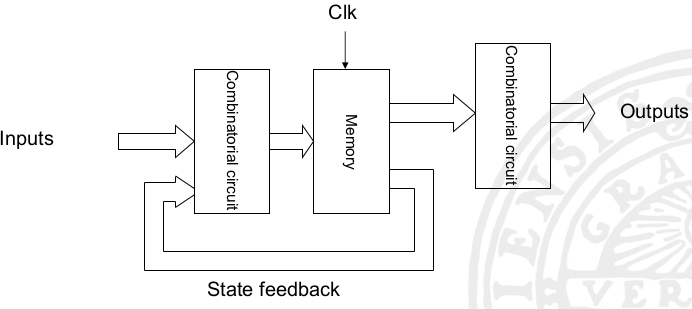
\includegraphics[width=12cm, height=6cm]{image/sequential-circuits-moore-type.png}
    \caption{Sequential circuits moore type}
\end{figure}

\begin{figure}[h]
    \vspace{10mm}
    \centering
    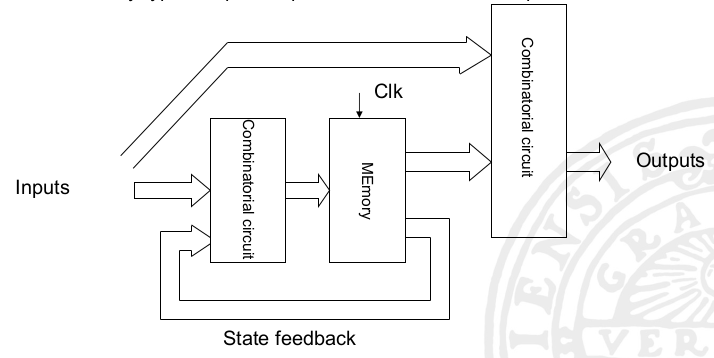
\includegraphics[width=10cm, height=6cm]{image/sequential-circuits-mealy-type.png}
    \caption{Sequential circuits mealy type}
\end{figure}

\newpage
\subsubsection{Memory}
\begin{table}[h!]
    \centering
    \begin{tabular}{ | m{5cm} | m{5cm} | }
        \hline
        Description & Circuit \\
        \hline
        SR-latch (memory cell)    
        &
        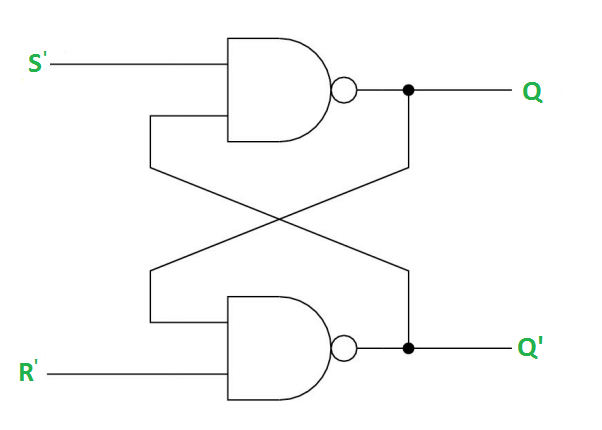
\includegraphics[width=0.3\textwidth]{image/SR_latch.png} \\
        \hline
        Gated SR-latch
        &
        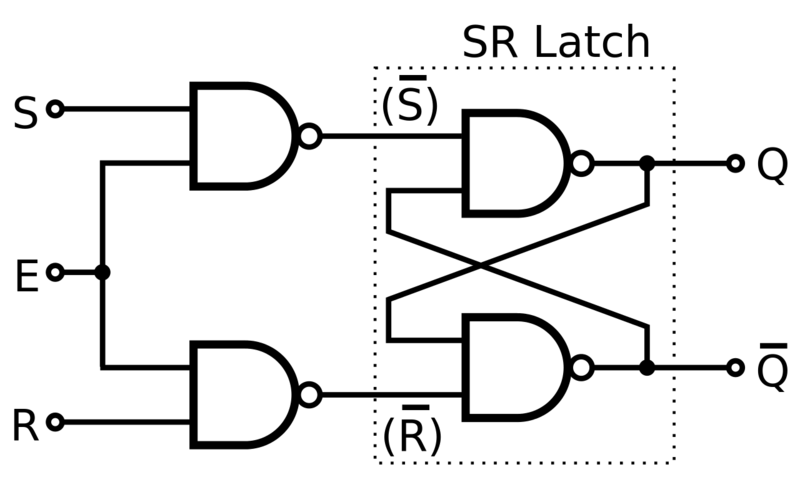
\includegraphics[width=0.3\textwidth]{image/Gated_SR_Latch.png} \\
        \hline
        Gated D-latch
        &
        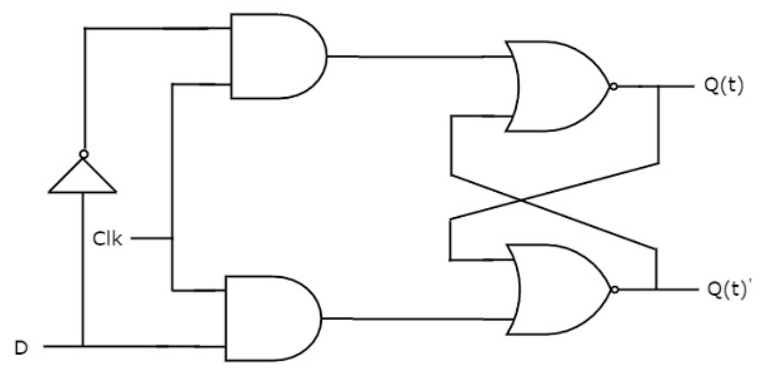
\includegraphics[width=0.3\textwidth]{image/Gated_D_latch.png} \\
        \hline
        D Flip Flops
        &
        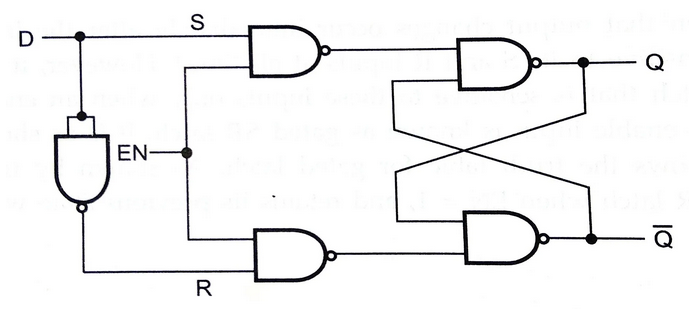
\includegraphics[width=0.3\textwidth]{image/D_Flip_Flop.png} \\
        \hline
    \end{tabular}
    \caption{Memory }\label{tbl:memory}
\end{table}

\newpage
\subsubsection{Timind diagram}
\begin{figure}[h]
    \vspace{10mm}
    \centering
    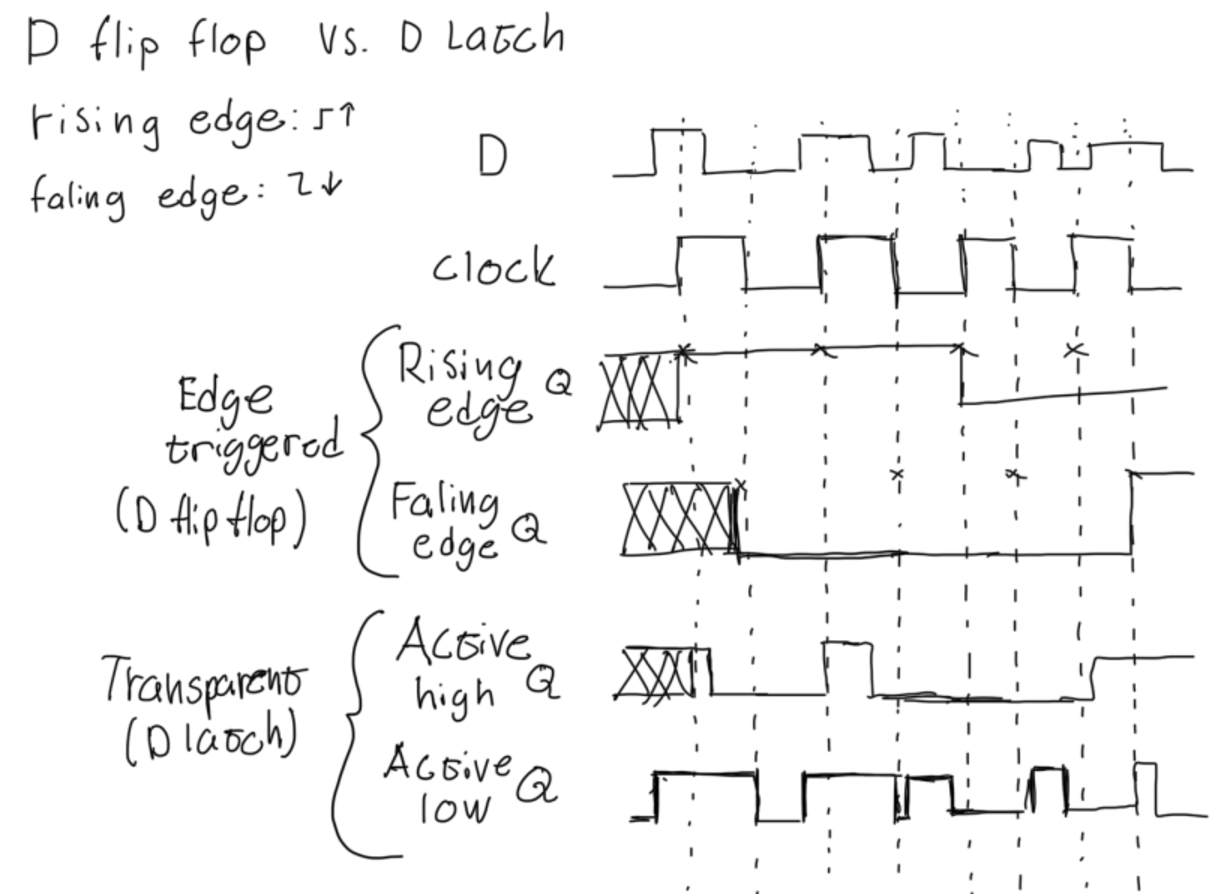
\includegraphics[width=10cm]{image/timing-diagram.pdf}
    \caption{Timing diagram}
\end{figure}


\subsubsection{State diagram}
\textbf{State code}
\begin{center}
\begin{tabular}{ | c | c c | }
    \hline
 State name & $q_1$ & $q_0$  \\ 
    \hline
 S0 & 0 & 0 \\
    \hline
 S1 & 0 & 1 \\
    \hline
 S2 & 1 & 0 \\
    \hline
 S3 & 1 & 1 \\
    \hline
\end{tabular}
\end{center}


\textbf{State Table}
In sequential circuits we use \textit{state table} instead of \textit{truth table}.
ex of state table format:
\begin{center}
\begin{tabular}{ | c | c | c | c | }
    \hline
 Previus state & Input & Next state & Output \\ 
    \hline
 0 0 & 0 & 0 0 & 0 \\ 
    \hline
 0 0 & 1 & 0 1 & 0 \\ 
    \hline
 0 1 & 0 & 0 1 & 1 \\ 
    \hline
 0 1 & 1 & 1 0 & 1 \\ 
    \hline
\end{tabular}
\end{center}

\newpage
\textbf{Moore-circuit}  
\begin{figure}[h]
    \centering
    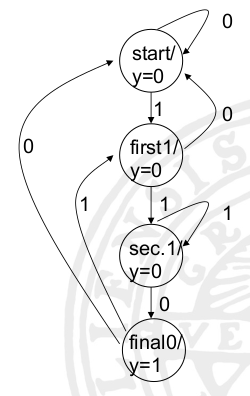
\includegraphics[width=5cm]{image/state-diagram-moore.png}
    \caption{State diagram moore}
\end{figure}
Note: in more machine we need a end state for output 1

\textbf{Mealy-circuit}  
\begin{figure}[h]
    \centering
    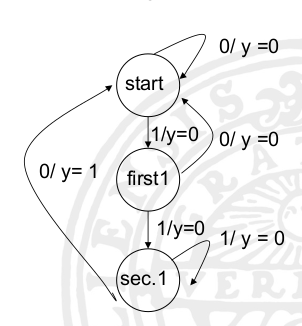
\includegraphics[width=5cm]{image/state-diagram-mealy.png}
    \caption{State diagram mealy}
\end{figure}
Note: in mealy machine we dont need that.




%mux memory element?
%reliable latch, ltaches
%2gate stratage only allow one 
%finate state mashine (FSM)
%state transition diagram
%(1) one input one output
%(2) ?all input and output

\newpage
\subsection{Shift registers}
Each pit is prosest simultaniusly. Makes much simpler circuit.
\begin{figure}[h]
    \centering
    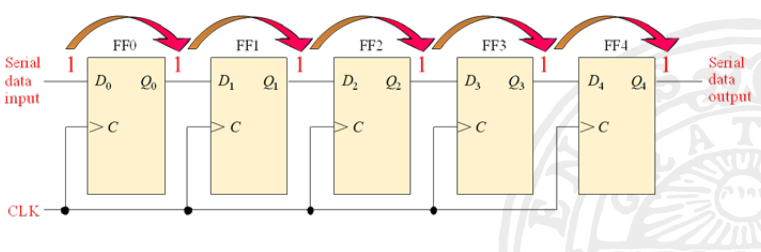
\includegraphics[width=10cm]{image/shift-register.png}
    \caption{Shift register}
\end{figure}

\subsection{Multiplixer}
$f(A,B,C)=\sum(0,1,5,6)$
\begin{figure}[h]
    \centering
    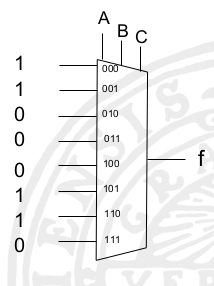
\includegraphics[width=5cm]{image/mux.png}
    \caption{Mux}
\end{figure}


\newpage
\section{AC Circuit Analysis \& Filtering}
Note: $G(\omega)=H(\omega)$

\begin{itemize}
    \item \textit{sinusoidal steady state} same as AC (analysis)
    \item \textit{phasor} a complex number representation of sinusoid 
    \item \textit{transfer function} relationsip with input and output voltage $G(jw)=\dfrac{v_{out}}{v_{in}}$
    \item \textit{Impedance} representation of $\dfrac{v_{in}}{i}$ (z)
    \item \textit{Angular frequency} $w=2\pi f$ where $f$ is frequency in $Hz$ with is cycles per second
    \item \textit{Operational frequency} $\frac{1}{\sqrt{2}}$
\end{itemize}

\begin{equation}
    v(t)=v_p\cos{wt+\phi}
\end{equation}

\textbf{Phasor \underline{3 representations}}
\begin{itemize}
    \item Rectangular form $z=x+jy$
    \item polar form $z=r \phase{\phi}$
    \item exponential form $z=ze^{j\phi}$
\end{itemize}

\textbf{Phasor conversion}
\begin{align*}
    r &= \sqrt{x^2+y^2} \\
    \phi &= \arctan{\frac{x}{y}} \\
    x &= r\cos(\phi) \\
    y &= r\sin(\phi) \\
    e^{j\phi} &= \cos{\phi} + j\sin{\phi} \\
    \cos\phi &= Re(e^{j\phi}) \\
    \sin\phi &= Im(e^{j\phi}) \\
\end{align*}

%\textbf{Rectangular to Polar}: $r=\sqrt{x^2+y^2}, \; \phi=\arctan{\frac{x}{y}}$
%\textbf{Polar to Rectangular}: $x=r\cos(\phi), \; y=r\sin(\phi)$

\textbf{Phasor operations}
\begin{align*}
    \text{addition: }& z_1+z_2 = (x_1+x_2)+j(y_1+y_2) \\
    \text{subtraction: }& z_1-z_2 = (x_1-x_2)+j(y_1-y_2) \\
    \text{multiplication: }& z_1z_2 = r_1r_2\phase{(\phi_1+\phi_2)} \\
    \text{division: }& \frac{z_1}{z_2} = \frac{r_1}{r_2}\phase{(\phi_1-\phi_2)} \\
    \text{inverse: }& \frac{1}{z} = \frac{1}{r}\phase{-\phi} \\
    \text{square root: }& \sqrt{z} = \sqrt{r}\phase{(\phi/2)} \\
    \text{complex conjugate: }& z^* = x-jy \\
\end{align*}

\textbf{Transfer function}
\begin{align*}
    H(j\omega) &= |H(j\omega)|\phase{H(j\omega)} \\
    H(w) &= \frac{v_o(w)}{v_i(w}
\end{align*}

\textbf{Euler formula}
\begin{align*}
    e^{jx}  &= \cos{x}+j\sin{x} \\
    e^{-jx} &= \cos{x}-j\sin{x} \\
    &\text{They are used to represent sinus wave.}
\end{align*}

We instead calculate with complex exponsetioals with euler formula instead of sinus waves
\begin{figure}[h]
    \centering
    \includegraphics[width=13cm]{image/AC-euler-representation-demostration.png}
    \caption{AC euler represent demostration}
\end{figure}

\vspace{10mm}
\textbf{AC Resistor representation}
\begin{figure}[h]
    \centering
    \includegraphics[width=13cm]{image/AC_resistor_representation.png}
    \caption{AC resistor represent}
\end{figure}


%Phasor representation
\newpage
\subsection{Impedance}
\textit{Impedance} $\dfrac{v_{in}}{i}$ (z)

\begin{align*}
  \textbf{Resistor}: &\quad \frac{v}{i}=R \\
  \textbf{Inductor}: &\quad \frac{v}{i}=jwl \\
  \textbf{Capasitor}: &\quad \frac{v}{i}=\frac{1}{jwc}\\
\end{align*}

%phasor transformations.
%transfer function!    (frequency ration (0 to 1) from the output vs input for voltage or current

%\begin{figure}[h]
%    \centering
%    \includegraphics[width=10cm, height=5cm]{image/transfer-function.png}
%    \caption{Transfer function}
%\end{figure}

%time domain vs frequnci domain.
%example of trasfer function

%frequency response, relationsip between input and output signal

\subsection{Filters}
The filter can eather be active and passive filters:
\begin{itemize}
    \item \textit{Passive filters} only use active components like resistor, capasitor and inductor
    \item \textit{Active filters} use opamp (can amplify output)
\end{itemize}

There are 4 common filtering types:
\begin{itemize}
    \item \textit{High-pass filter (HP)} lets higher frequencys threow
    \item \textit{Low-pass filter (LP)} lets lower frequencys threow
    \item \textit{Bandpass filter (BP)} within a frequency spand. Can be comind with HP and LP in series
    \item \textit{Notch filter} oposit of BP
\end{itemize}
\begin{figure}[h]
    \vspace{10mm}
    \centering
    \includegraphics[width=10cm]{image/signal-filtering.png}
    \caption{Signal filtering}
\end{figure}


Filters can be constructed as follows: \newline
\textit{RC filter}, \textit{RL Filter}, \textit{LC filter}, 
\textit{L-filter}, \textit{$\pi$-filter} and \textit{T-filter}.

\newpage
\textbf{Some resorces to construct filters}
\begin{itemize}
    \item \href{https://rf-tools.com/lc-filter/}{RF tools}
    \item \href{https://tools.analog.com/en/filterwizard/}{Filterwizard}
\end{itemize}

\textbf{Example: HP filter}
\begin{figure}[h]
    \centering
    \includegraphics[width=10cm]{image/HP-filter_circuit.png}
    \caption{HP Filter Circuit.png}
\end{figure}
\begin{align*}
    V_{out} &\quad = V_{in}\dfrac{z_R}{z_C+z_R} \;\;\; 
           \text{ -From voltage divider circuit} \\
           &\quad = V_{in}\dfrac{R}{\frac{1}{j\omega c}+R} \;\;\; \text{ -From impedance axiom} \\
           &\quad = V_{in}\dfrac{\frac{R}{1}}{\frac{R(j\omega c)+1}{j\omega c}} 
           = V_{in}\dfrac{R(j\omega c)}{R(j\omega c)+1}  \\
\end{align*}
Therefore we get $G_{HP}=\dfrac{R(j\omega c)}{R(j\omega c)+1}$

\begin{align*}
|G_{HP}| &=\dfrac{1}{\sqrt{2}}=\dfrac{R\omega c}{\sqrt{R^2\omega^2c^2+1}} \\
         &\Rightarrow \dfrac{\sqrt{R^2\omega^2c^2+1}}{\sqrt{2}}=R\omega c \\
         &\Rightarrow \dfrac{R^2\omega^2c^2+1}{2}=R^2\omega^2c^2 \\
         &\Rightarrow R^2\omega^2c^2+1=2R^2\omega^2c^2 \\
         &\Rightarrow R^2\omega^2c^2=1 \\
         &\Rightarrow R\omega c=1 \\
         &\Rightarrow R=\frac{1}{\omega c} \\
\end{align*}
The following is given: $\omega=2\pi f$, $1kHz$ for HP filter.
The capacitor should not be larger than $2.2uF$.
Therefore we chose $c=1uF$, this gives us $R\approx 160\Omega$.

\begin{align*}
    &arg(G_{HP})=arg(\dfrac{160 \cdot 2 \cdot \pi \cdot 10^-6 \cdot f \cdot j}{160 \cdot 2 \cdot \pi \cdot 10^-6 \cdot f \cdot j + 1}) \\
    &= arg(160 \cdot 2 \cdot \pi \cdot 10^-6 \cdot f \cdot j) - arg(160 \cdot 2 \cdot \pi \cdot 10^-6 \cdot f \cdot j + 1)\\
    &=\dfrac{\pi}{2} - arctan(\dfrac{160 \cdot 2 \cdot \pi \cdot 10^-6 \cdot f}{1})\\
    &=\dfrac{\pi}{2} - arctan(\dfrac{\pi \cdot f}{3125})
\end{align*}

\begin{align*}
    &arg(G_{HP})=arg(\dfrac{160 \cdot 2 \cdot \pi \cdot 10^-6 \cdot f \cdot j}{160 \cdot 2 \cdot \pi \cdot 10^-6 \cdot f \cdot j + 1}) \\
    &\Rightarrow \dfrac{z_1}{z_2} = \frac{r_1}{r_2}\phase{\phi_1-\phi_2}  \\
    &\Rightarrow \dfrac{z_1}{z_2} = \frac{\sqrt{(0.32 \cdot 10^{-3} \cdot f\pi)^2}}{\sqrt{(0.32 \cdot 10^{-3} \cdot f\pi)^2 + 1}}\phase{\arctan{0}-\arctan{\frac{1}{0.32 \cdot 10^{-3} \cdot f\pi}}}  \\
    &\Rightarrow arg(\dfrac{z_1}{z_2}) = -\arctan{\frac{1}{0.32 \cdot 10^{-3} \cdot f\pi}}  \\
    &= -\arctan{\frac{1}{0.32 \cdot 10^{-3} \cdot f\pi}}  \\
    &= \frac{\pi}{2}-\arctan{\frac{f\pi}{3125}}  \\
\end{align*}


\textbf{Example: exponential representation}
\begin{align*}
    H(j\omega) &= \frac{j\pi}{1+j2\pi} = |H(j\omega)| e^{j arg(H(j\omega))} \\
    \Rightarrow &|H(j\omega)| = \frac{\sqrt{\pi^2}}{\sqrt{1^2+2^2\pi^2}}
    = \frac{\pi}{\sqrt{1+4\pi^2}} \\
    &\\
    &arg(H(j\omega)) = arg\Big(\frac{j\pi}{1+j2\pi}\Big)= \arctan{\Big(\frac{0}{\pi}\Big)}-\arctan{\Big(\frac{1}{2\pi}\Big)} \\
    &= \frac{\pi}{2} -\arctan{\Big(2\pi\Big)} \\
    \Rightarrow &H(j\omega) = \frac{\pi}{\sqrt{1+4\pi^2}}e^{j\arctan{\Big(2\pi\Big)}} \\
\end{align*}

\subsubsection{Series of filter}
One can \underline{commbind filters} to create more complex filters.
The \textit{transfer function} will be the \underline{multiplication} of 
\begin{equation}
    G_{tot} = G_{1}\cdot{G_2}\cdot \ldots \cdot{G_n}
\end{equation}
The \textit{Gain} will be the \underline{gain} for each \underline{individual} transfer function \underline{multiplied}
\begin{equation}
    |G_{tot}| = |G_{1}|\cdot|{G_2}|\cdot \ldots \cdot|{G_n}|
\end{equation}
The phase function is the sum of the phase functions
\begin{equation}
    Arg(G_{tot}) = Arg(G_{1})+Arg({G_2})+\ldots+Arg(\cdot{G_n})
\end{equation}


%example 12 assignment.
%example 8 assignment

